
\subsection{Funnels}
\label{sec:funnels}

The uncertainty guarantees in this thesis is made through creating
\textit{funnels}. Funnels are the parameterization of the \textit{finite time
  reachable sets} for the dynamical system at hand. The following sections will
introduce and develop the theory needed to understand the \ac{SOS} framework
that lies at the bottom of the mathematical verification of these reachable
sets. For the curious reader, a more basic introduction can be found in
\cref{sec:first-app}.

A \textit{funnel} is a parameterization of the reachable set of a dynamical
system. This means that a Funnel holds all the states the dynamical system can
be in during a planning task. Mathematically the reachable set of the system is
defined as
\[
  \vect{x}(0) \in \mathcal{X}_0 \implies \vect{x}(t) \in F(t), \forall t \in
  \sqb{0,T},
\]
where \(\mathcal{X}_0\) is the set of initial conditions, \(\sqb{0,T}\) the time
interval, and \(F(t)\) is the set of states that the system can be in at time
\(t\). Although this thesis concerns itself with approximating the reachable set
through \textit{Lyapunov} functions, a useful analogy is imagining the funnel
created through \textit{Monte-Carlo} simulation, where the funnel would be the
set of all the paths traversed by the dynamical system at hand. For the simple
airplane model \cref{eq:model-dynamics}, a Monte-Carlo simulation of nine
starting points along the y-axis, along with a simple \ac{LQR} controller on the
heading of the aircraft, can be seen in \cref{fig:monte-carlo-sim}.

\begin{figure}[!t]
  \centering 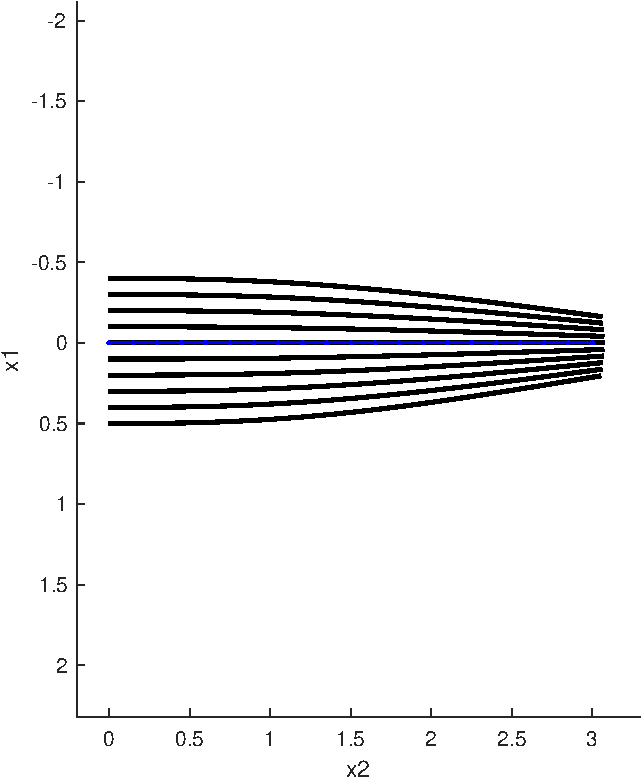
\includegraphics[scale=.6]{figures/preliminaries/montecarlofunnel}
  \caption[Monte-Carlo simulation of the funnel for the \ac{LQR}-controller]{The simulation of N paths starting from a random point in the
    interval \(\sqb{-.5,.5}\), and controlled with a LQR controller.}
  \label{fig:monte-carlo-sim}
\end{figure}

In the literature, the term funnel first appears in
\cite{masonMechanicsManipulation1985}, but is later employed in a lot of
research. The funnel definitions in this thesis is taken from a series of
articles on funnels~\cite{Tobenkin_2011,tedrakeLQRtreesFeedbackMotion2009,
  majumdarRobustOnlineMotion2013,
  majumdarFunnelLibrariesRealtime2017,ahmadi2014dsos}, with the main focus being
on \cite{majumdarFunnelLibrariesRealtime2017}.


\subsection{Computing Funnels}

The funnel computations will be based on the \ac{SOS} theory developed in the
following sections. When given a nominal trajectory, the goal is to compute a
robust invariant set around this trajectory that will guarantee that the planner
is free from collisions during execution of the obtained motion plan. This
robustly invariant set is parameterized through Lyapunov function candidates,
that, in this case, will be based upon an \ac{LQR} controller for the system.

In order to compute funnels, a model of the dynamics for the system is required.
Thus, given the nonlinear dynamical system
\begin{equation}
  \label{eq:dynamicalsystem}
  \dot{\vect{x}} = f\big(\vect{x}(t), \vect{u}(t) \big),
\end{equation}
with \(\vect{x}(t)\) the state of the system at time \(t\), and \(\vect{u}(t)\)
the control input. Assume that an open loop nominal trajectory \(\vect{x}_0
\colon [0,T] \rightarrow \R^n\) with control input \(\vect{u}_0 \colon [0,T]
\rightarrow \R^n\) is given, and define a change of coordinates into the error
coordinate frame
\begin{align}
  \label{eq:system-error-dynamics}
  \bar{\vect{x}}(t) &= ( \vect{x} - \vect{x}_0 )(t) \\
  \bar{\vect{u}}(t) &= (\vect{u} - \vect{u}_0 )(t) \mathEoS
\end{align}
Then, transforming \cref{eq:dynamicalsystem} to the new coordinate frame one
obtains
\begin{equation}
  \label{eq:dynamicalsystem-coordinatechange}
  \dot{\bar{\vect{x}}} = \dot{\vect{x}} - \dot{\vect{x}}_0 = f\big( \vect{x}_0(t) + \bar{\vect{x}}(t), \vect{u}_0(t) + \bar{\vect{u}}(t) \big) - \dot{\vect{x}}_0(t) \mathEoS
\end{equation}

In order to compute a parameterized reachable set through \ac{SOS} programming
the system~\cref{eq:dynamicalsystem-coordinatechange} needs to be polynomial,
and parameterized by \(\vect{x}\) and \(t\) polynomially, since the \ac{SOS}
framework can only verify polynomial inequalities. Therefore, through the use of
a \ac{TV-LQR} (although any controller providing a \ac{CLF} can be used), the
control input can be eliminated from the dynamical equation, giving
\begin{equation}
  \label{eq:dynamicclosedloop}
  \dot{\bar{\vect{x}}} = f_{cl}\big( t,\bar{\vect{x}}(t) \big) \mathEoS
\end{equation}
However, the dynamical system may still not be polynomial, which is a necessary
condition in order for the system to be verified using \ac{SOS} programming.
Therefore, by expanding the system in \cref{eq:dynamicclosedloop} around the
nominal trajectory \(\vect{x}_0\), through a Taylor polynomial of some degree
\(N\), the resulting polynomial should be able to capture the nonlinearities of
the system.

The goal is to parameterize a \textit{tight outer approximation} of the set of
states the system may transition into during the time interval \([0,T]\). Given
that \(F(t)\) is the set of states the system~\cref{eq:dynamicclosedloop} can be
in at time \(t\), then
\begin{equation}
  \label{eq:reachableset}
  \bar{\vect{x}}(0) \in \mathcal{X}_0 \implies \bar{\vect{x}}(t) \in F(t), \, \forall t \in [0,T],
\end{equation}
where \(\mathcal{X}_0\) is the initial condition set, and \(F(t) \subset \R^n\)
is the finite time funnel for the system.

\begin{definition}
  \label{def:funnel}
  A funnel associated with a closed-loop dynamical system \(\dot{\bar{\vect{x}}}
  = f_{\mathit{cl}}\big( t,\vect{x}(t) \big) \) is a map \(F \colon [0,T]
  \rightarrow \mathcal{P}(\R^n)\), from the time interval \([0,T]\) to the power
  set (i.e., the set of subsets) of \(\R^n\) so that the sets \(F(t)\) satisfy
  the
  condition~\cref{eq:reachableset}~\cite{majumdarFunnelLibrariesRealtime2017}.
\end{definition}

Next, the reachable set is parameterized through the use of Lyapunov functions,
which yields
\begin{equation}
  F(t) = \set{\bar{\vect{x}}(t) \mid V \big(t, \bar{\vect{x}}(t) \leq \rho (t) \big)},
\end{equation}
where \(\rho (t) \colon [0,T] \rightarrow \R^+\), is an upper bound which limits
the size of the reachable set, and \(V \big(t,\bar{x}(t) \big)\) is a Lyapunov
function \(V \colon [0,T] \times \R^n \rightarrow \R^+\).

Then, by setting \(\mathcal{X}_0 \subset F(0,\bar{\vect{x}})\), one can derive
the sufficient condition~\cref{eq:reachableset} for containing the reachable set
in the Lyapunov function parameterization
\begin{equation}
  \label{eq:funnelsufficient}
  V(t,\bar{\vect{x}}) = \rho(t) \implies \dot{V}(t,\bar{\vect{x}}) < \dot{\rho}(t), \, \forall t \in [0,T], 
\end{equation}
with \(\dot{V}(t,\bar{\vect{x}})\) computed as
\begin{equation}
  \dot{V}(t,\bar{\vect{x}}) = \frac{\partial V(t,\bar{\vect{x}})}{\partial \vect{x}} f_{\mathit{cl}}(t,\bar{\vect{x}}) + \frac{\partial V(t,\bar{\vect{x}})}{\partial t} \mathEoS
\end{equation}

Currently there are no limitations on the functions \(V\) and \(\rho\), and
hence there exists infinitely many functions with different sized reachable sets
that satisfies~\cref{eq:funnelsufficient}, and is a valid funnel in the sense of
~\cref{def:funnel}. In order for efficient planning to take place, the motion
primitives, meaning the size of the funnels, should be as small as possible, and
it is therefore that the volume of the funnels is minimized using the following
optimization problem

\begin{align}
  \label{eq:funneloptimizationproblem}
  &\underset{V,\rho}{\text{infimum}} \; &&\int_{0}^{T} \vol\big( F(t) \big) \, \mathrm{d}t \\
  &\text{subject to} && V(t,\bar{\vect{x}}) = \rho (t) \implies \dot{V}(t,\bar{\vect{x}}) < \rho (t) \, \forall t \in [0,T] \label{eq:funnel-optimization-subject-to} \\
  && &\mathcal{X}_0 \subset F(0,\bar{\vect{x}}) \mathEoS \nonumber
\end{align} 

\begin{figure}
  % \centering
  % \includegraphics[scale=.7]{figures/experiments/lyapunov_visualization}
  \centering { \fontsize{16pt}{16pt}\selectfont \def\svgwidth{.8\textwidth}
    \import{figures/experiments/}{lyapunov_visualization.pdf_tex} }
  \caption[A converging funnel parameterized through a Lyapunov function]{A visualization of the Lyapunov function along a trajectory, where
    the center of the Lyapunov function moves along the trajectory with time
    \(t\).}
\end{figure}


\subsection{Formulating the Optimization Problem as a SOS Program}

The optimization problem in \cref{eq:funneloptimizationproblem} would not be
impossible to solve efficiently had it not been for advances in mathematical
convex numerical optimization by
\citeauthor{parilloStructuredSemidefinitePrograms}~\cite{parilloStructuredSemidefinitePrograms},
as in general the problem involves searching over an infinite function space.
While the general optimization problem of searching through an infinite function
space is not amenable to efficient numerical computation, the problem can be
made computationally feasible through the use of a \ac{SOS} programming
approach~\cite{tedrakeLQRtreesFeedbackMotion2009}.

Thus in order to make the problem amenable to a \ac{SOS} program, there are a
few requirements that need to be met by the problem formulation. Firstly the
initial condition set needs to be a \textit{semi-algebraic set}, (i.e.,
parameterized by polynomial inequalities) so that
%
\begin{equation}
  \label{eq:initial-condition-set-parameterized}
  \mathcal{X}_0 = \set{\bar{\vect{x}} \in \R^n \mid g_{o,i}(\bar{\vect{x}}) \geq 0, \, i = 1,\ldots,N_0},
\end{equation}
%
is the initial condition set. Then rewriting \cref{eq:funnelsufficient} in terms
of positivity and equality constraints yields
\begin{equation}
  V(t,\bar{\vect{x}}) = \rho(t) \implies \dot{\rho}(t) - \dot{V}(t,\bar{\vect{x}}) > 0,
\end{equation}
and the initial condition set \eqref{eq:initial-condition-set-parameterized} is
rewritten
\begin{equation}
  g_{0,i}(\bar{\vect{x}}) \geq 0 \, \forall i \in \set{1,\ldots,N_0} \implies \rho(0) - V(0,\bar{\vect{x}}) \geq 0 \mathEoS
\end{equation}
Which, if these functions are both polynomial, is now in the form of a \ac{SOS}
optimization problem. Then through the use of the \nameref{sec:s-procedure} one
can write the optimization problem~\eqref{eq:funneloptimizationproblem} as
\begin{subequations}
\begin{align}
  \dot{\rho}(t) - \dot{V}(t,\bar{\vect{x}}) - L(t,\bar{\vect{x}}) \big( V(t,\bar{\vect{x}}) - \rho(t) \big)& \nonumber \\
                                            - L_{t}(t,\bar{\vect{x}})\big( t\left( T - t \right) \big)&   \label{eq:sufficient-conditions}
  &\text{is SOS}&  \\
  \rho(0) - V(0,\bar{\vect{x}}) - \sum_{i}^{N_{0}} L_{0,i}(\bar{\vect{x}})g_{0,i}(\bar{\vect{x}})&  &\text{is SOS}& \label{eq:sufficient-conditions-2} \\
  L(t, \bar{\vect{x}}), \, L_{t}(\bar{\vect{x}}), \, L_{0,i}(\bar{\vect{x}})& &\text{are SOS}&, \nonumber \\
  &&\forall i \in \set{1,\ldots,N_{0}},& \nonumber
\end{align} 
\end{subequations}
where \(L\), \(L_{t}\), and \(L_{0,i}\) are multiplier polynomials~(see
\cref{sec:s-procedure}).

The goal is to make the parameterization of the reachable set as small as
possible, and therefore minimizing the cost function in
\cref{eq:funneloptimizationproblem}. This is done by \textcite{Tobenkin_2011}
through approximating the cost function by first discretizing the problem and
replacing the integral with a finite sum
\begin{equation}
  \int_{0}^{T} \vol\big( F(t) \big) \, \mathrm{d}t \rightarrow \sum_{k=1}^{N} \vol\big( F(t_{k}) \big) \mathEoS \label{eq:discrete-costfunction}
\end{equation}
Since the Lyapunov function \(V(t,\bar{\vect{x}})\) in this thesis is quadratic,
it can be written as
\begin{equation}
  V(t_{k}, \bar{\vect{x}}) = {\bar{\vect{x}}}^{T}S_{k}\bar{\vect{x}}, \, S_{k} \succeq 0,
\end{equation}
where \(\succeq 0\) means that the matrix is positive semi-definite. Since the
set \(F(t_{k})\) is now an ellipsoid in which the volume can be minimized
through maximizing the determinant of \(S_{k}\), which in turn can be
transformed into a \acl{SDP} problem (see \cref{subsec:sdp}). If an upper bound
on the cost function \cref{eq:discrete-costfunction} is introduced as
\begin{equation}
  \mathcal{E} (t_{k}) = \set{\bar{\vect{x}} \in \R^n \mid {\bar{\vect{x}}}^{T}S_{k}\bar{\vect{x}} \leq 1, \, S_{k} \succeq 0},
\end{equation}
where \( \mathcal{E} ( t_{k} ) \) is an ellipsoid containing the reachable set
\( F ( t_{k} ) \) at time \( t_{k} \). This containment constraint can be
equivalently expressed as
\begin{equation}
  V ( t_{k}, \bar{\vect{x}} ) \leq \rho(t_{k})  \implies {\bar{\vect{x}}}^{T}\matr{S}_{k}\bar{\vect{x}} \leq 1 \mathEoS
  \label{eq:discrete-containment-constraint}
\end{equation}
Which when expressed using \ac{SOS} constraints gives
\begin{align}
  1 - {\bar{\vect{x}}}^{T}\matr{S}_{k}\bar{\vect{x}} - L_{\mathcal{E},k}(\bar{\vect{x}}) \big( \rho(t_{k}) - V(t_{k}, \bar{\vect{x}}) \big)  \qquad \text{is SOS}& \\
  L_{\mathcal{E},k}(\bar{\vect{x}}) \qquad \text{is SOS}& \mathEoS \nonumber
\end{align}
%
Then combining the cost function~\eqref{eq:discrete-costfunction} with the
constraints in Equation~\eqref{eq:discrete-containment-constraint} along with
\cref{eq:sufficient-conditions,eq:sufficient-conditions-2}, one arrives at the
following optimization problem:
  \newcommand{\E}{\mathcal{E}}
  \begin{mini!}[2]
    { \substack { V, \rho, L, L_t,
        \\
        L_{0, i}, S_{k}, L_{\E, k} } }
    { \sum_{k = 1}^{N} \vol \bigl( \E(t_{k}) \bigr) =
      \sum_{k = 1}^{N} \vol \bigl( \set{\vect{x} \mid \vect{x}^{T} \matr{S}_{k} \vect{x}
        \le 1} \bigr) }
    {\label{opt:time-dependent-optimization-problem}}
    {}
    \addConstraint {
        \dot{\rho}(t) -
      \dot{V}(t,\vect{x}) - L(t,\vect{x}) \bigl( { V(t,\vect{x}) - \rho(t) }
      \bigr) \nonumber }
    {}
    {}
    \addConstraint{- L_t (t,\vect{x}) \bigl(  {t \p*{T - t}} \bigr) }
    {}
    {\text{ is SOS}}
    \addConstraint {\rho(0) - V(0, \vect{x}) - \sum_i^{N} L_{0,
        i}(\vect{x}) g_{0, i}(\vect{x}) }
    {}%
    {\text{ is SOS}}
    \addConstraint { 1 - \vect{x}^T \matr{S}_k \vect{x} -
      L_{\E, k}(\vect{x}) \bigl(  {\rho(t_k) - V(t_k, \vect{x})} \bigr) }
    {}%
    {\text{ is SOS}}
    \addConstraint {S_k \nonumber}%
    {\succeq 0}%
    {\quad \forall k \in \set{1, \ldots, N}}
    \addConstraint {L(t,\vect{x}), L_t (t, \vect{x}),\, L_{0,i}(\vect{x}),\,
      L_{\mathcal{E},k}(\vect{x}) \nonumber }%
    {\qquad\text{ are SOS}}%
    {\quad \forall i \in \set{1, \ldots, N_0},}
    \addConstraint{\nonumber}{}{\quad \forall
      k \in \set{1, \ldots, N} \mathEoS }
  \end{mini!}
This is the continuous finite dimensional optimization problem that is needed in
order to search for a Lyapunov function candidate that parameterizes the
reachable set for the dynamical system at hand.

However, this optimization problem is not in general convex, as the first
constraints are \textit{bilinear} in the decision variables, since \(L\) and
\(V\) are multiplied together. However, the problem can be solved, although not
optimally, if \(V\) and \(\rho\) are held fixed, while the other decision
variables are free. Likewise, fixing \(L\) and \(L_{\mathcal{E},k}\), creates
another \ac{SOS} optimization program. Therefore shifting between the two sets
of decision variables \(\left( L,L_{t},L_{0,i},L_{\mathcal{E},k} \right) \) and
\(\left( V,\rho,L_{0,i},\matr{S}_{k} \right) \)
\textcite{majumdarFunnelLibrariesRealtime2017} arrives at
\cref{alg:funnelalgorithm} on page~\pageref{alg:funnelalgorithm} for computing
funnels.

\begin{algorithm}[H]
  \caption{Funnel computation}
  \label{alg:funnelalgorithm}
  \begin{algorithmic}[0]
    \Procedure{FunnelComputation}{\(V,\rho\)}
    \State Output: Funnel
    \State \(\mathnormal{cost}_{\mathnormal{prev}} = \infty\)
    \State converged = false
    \While {\( \neg \mathnormal{converged}\)}
    \State Optimization Problem 1:
    \State %
    \begin{align*}
      \underset{\substack{L,L_{t},L_{0,i},S_{k},L_{}}}{\inf}&  \sum_{k=1}^{N} \vol \bigl( \mathcal{E}(t_{k}) \bigr) & \\    
      \text{subject to } & V \text{ and } \rho \text{ constant.}& \\
    \end{align*}
    \State Optimization Problem 2:
    \State %
    \begin{align*}
      \underset{\substack{V,\rho, L_{t},L_{0,i},S_{k}}}{\inf}&  \sum_{k=1}^{N} \vol \bigl( \mathcal{E}(t_{k}) \bigr) & \\    
      \text{subject to } & L \text{ and } L_{\mathcal{E},k} \text{ constant.}& \\
    \end{align*}
    \State 
    \State cost = \(\sum_{k=1}^{N} \vol \bigl( \mathcal{E}(t_{k}) \bigr) \)
    \State
    \If{\(\frac{\mathrm{cost}_{\mathit{prev}} -
    \mathrm{cost}}{\mathrm{cost}_{\mathit{prev}}} < \epsilon \) }
    \State converged = true
    \EndIf
    \State \(\mathrm{cost}_{\mathit{prev}} = \mathrm{cost}\)
    \EndWhile
    \EndProcedure
  \end{algorithmic}
\end{algorithm} 